\documentclass[a4paper,11pt]{article}

\usepackage[hidelinks]{hyperref}
\usepackage[font={small}]{caption}
\usepackage{graphicx}
\usepackage[lined,boxed]{algorithm2e}
\usepackage{algpseudocode}
\usepackage{mathtools}
\usepackage{poltakmacros}           % Personal macros included in file 'poltakmacros.sty'.
\usepackage{geometry}

\geometry{margin=2cm}


\author{Jonathan Poltak Samosir}
\title{FIT3143 Assignment 2}


\begin{document}

\maketitle
\thispagestyle{empty}

\begin{abstract}
\end{abstract}
\smallskip
\noindent \textbf{Keywords.} blah, blah, blah
\newpage
\pagenumbering{roman}
\tableofcontents
\newpage

\pagenumbering{arabic}

% TODO: Split sections into different files
\section{Introduction} % (fold)
\label{sec:introduction}

% section introduction (end)


\section{Introduction to the multi-core CPU} % (fold)
\label{sec:introduction_to_the_multi_core_cpu}

\subsection{The central processing unit} % (fold)
\label{sub:the_central_processing_unit}
The central processing unit --- hereby referred to as the CPU --- is a fundamental piece of hardware within modern computers that handles
the fetching, decoding and execution of each instruction of a computer program~\cite{web:CPUWiki}. It handles the processing
of these instructions through the use of two key components: the arithmetic logic unit --- hereby referred to as the ALU
--- for basic arithmetical and logical operations, and the control unit --- hereby referred to as the CU --- for the input/output
operations between the CPU and memory, along with the overall control of the fetch, decode and execute cycle. Given the
physical hardware constraints, only a single instruction may be processed at any given time by a CPU.
% subsection the_central_processing_unit (end)

\subsection{The multi-core CPU} % (fold)
\label{sub:the_multi_core_cpu}
To define the multi-core CPU, it is perhaps important to first define the term ``core''. Like many terms in the area of computing,
the term ``core'' is often misused or used with many different meanings attached to it. For the purposes of this paper, the
term ``core'' simply refers to actual CPUs as defined in~\sectref{sub:the_central_processing_unit}.

Given this definition of a core, the multi-core CPU can simply be defined as a piece of computing hardware that contains
two or more cores. As the multi-core CPU contains more than one core, rather than being constrained to processing a single
instruction at any given time, in theory it is possible to be processing $n$ instructions on an $n$-core CPU at any given time.

Given what multi-core CPU hardware makes possible, since their introduction to consumers in the early 2000s, the multi-core
CPU has changed the way programmers design their programs to take advantage of hardware. Programs that are designed with
code concurrency in-mind now have advantages that were only ever available previously on systems that have multiple physical
CPU chips.
% subsection the_multi_core_cpu (end)

\subsection{Multi-core CPU architecture} % (fold)
\label{sub:multi_core_cpu_architecture}
The newest evolutions in multi-core CPU architecture families in modern consumer computing are arguably Intel's
``Haswell'' and AMD's ``Steamroller'' lines of processors.

Intel's Haswell is the fourth generation of their ``Core'' line of multi-processors, that places a larger focus on reducing power-consumption and improving performance of their on-chip graphics processing unit, or GPU~\cite{web:ForbesHaswell}. This point, specifically, will be elaborated on in further detail in later sections.

AMD's Steamroller architecture is the third evolution of AMD's ``Bulldozer''
architecture, a direct competitor to Intel's Haswell architecture implemented
in their ``Core'' line of multi-core processors. Steamroller placed a larger focus on improving parallelism between the available cores~\cite{web:AMDCCCSlides}, while also attempting to address competitor Intel's area of dominance--- power
consumption.
% subsection multi_core_cpu_architecture (end)

\subsubsection{Intel Haswell Core i7-4770K architecture} % (fold)
\label{subsub:intel_haswell_architecture}
As an example of a Haswell CPU to specifically look at, we will take Intel's
current flagship enthusiast model Haswell quad-core processor, the Core i7-4770K. While having four cores all on the same chip, this Core i7 also
contains its own GPU on the chip. The Haswell i7 is a multi-level cache CPU, with each core having three levels of cache memory
available to it; from fastest to slowest: L1, L2 and L3. Each core has its own
dedicated 64 KB of L1 cache (split into 32 KB halves for separate data and instruction caches), 256 KB of L2 cache and all the cores share a much slower 8 MB of L3 cache~\cite{web:TomsHWCorei7}. The overall layout of the chip, as explained here, can be seen in~\figref{fig:haswell-layout}.

\begin{figure}[ht]
  \centering
  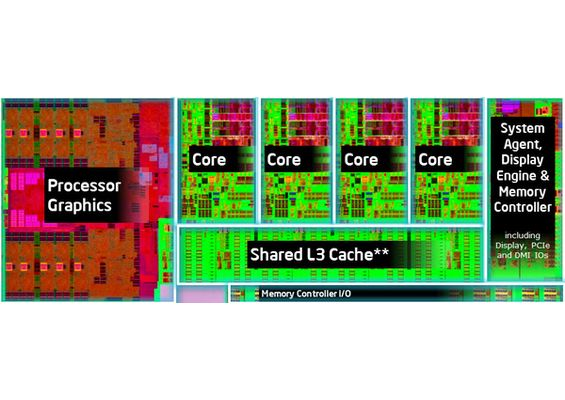
\includegraphics[scale=0.5]{img/haswell-layout}
  \caption{The Intel Core i7-4770K quad-core CPU die layout.~\cite{web:TomHWCorei7DiePic}}
\label{fig:haswell-layout}
\end{figure}

Something of note is how the i7-4770K enables pipelining of operations with its hardware. Before proceeding into pipeling, it is important to touch on the differences between instructions and operations: Instructions are decoded by the CPU into atomic parts which are known as micro-operations which use and require specific resources. These micro-operations are then queued into the ``Unified Reservation Station'' (URS) where they wait until their resources are available. The micro-operations are then dispatched from the URS to the appropriate execution port. This is all done ``out of order'' where operations are just dispatched whenever possible, rather than in a pre-determined order when there is no resource dependencies between operations~\cite{book:Corei7PerfAnalysis}. Hence, this is the specific implementation of CPU pipelining that is enabled on the Haswell architecture. As can be seen from~\figref{fig:haswell-new-ports}, Haswell has eight distinct execution ports, each supporting different operations. This allows a maximum of eight independent micro-operations to be executed each clock cycle~\cite{web:TomsHWCorei7}.

\begin{figure}[ht]
  \centering
  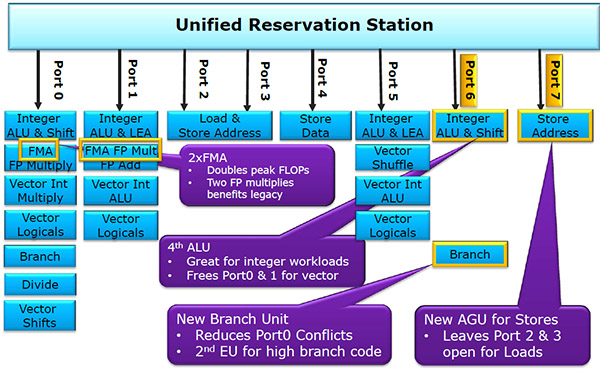
\includegraphics[scale=0.5]{img/new-ports}
  \caption{Shows how operation out of order execution pipelining works in the Intel Core i7-4770K~\cite{web:TomsHWCorei7}. The Unified Reservation Station can be seen along with the i7's eight execution ports. New hardware additions to the Haswell architecture highlighted.}
\label{fig:haswell-new-ports}
\end{figure}
% subsection intel_haswell_architecture (end)

\subsubsection{AMD Steamroller/Kaveri architecture} % (fold)
\label{subsub:amd_steamroller_architecture}
As an example of a Steamroller-based CPU, we will look at AMD's current flagship A10-7850K processor, which is based on the third evolution of the Steamroller architecture, codenamed ``Kaveri''.

Something of note when looking at modern AMD processors is to note AMD's use of the marketing term ``APU'' --- short for Accelerated Processing Unit. This is essentially AMD's term for a GPU and CPU dual-offering on the same die~\cite{web:AMDAPU}, similar to what is provided by Intel's Haswell line of processors (as elaborated on in~\sectref{subsub:intel_haswell_architecture}).

Like the Haswell i7, the Kaveri processors have four cores. Unlike the Haswell, the cores are split into two distinct ``dual-core'' units (each, of course, housing two separate cores). As the Kaveri line are also multi-level cache processors, each dual-core unit has its own L1 and L2 cache. The L1 cache is split into a 96 KB instruction cache for each dual-core unit and four separate 16 KB of data cache reserved for each of the cores~\cite{web:Guru3dKaveri}. The L2 cache is 2 MB large for each dual-core unit. Unlike the Haswell processors, there is no L3 cache present.

Like the cache architecture, the die layout for the Kaveri processors, seen in~\figref{fig:kaveri-layout}, is quite different to what we have previously seen with Intel's Haswell processors. The most obvious difference is that the majority of the die is taken up by the GPU. This shows AMD's larger emphasis on competitive graphics with their ``APU'' direction~\cite{web:WikiAPU}.

\begin{figure}[ht]
  \centering
  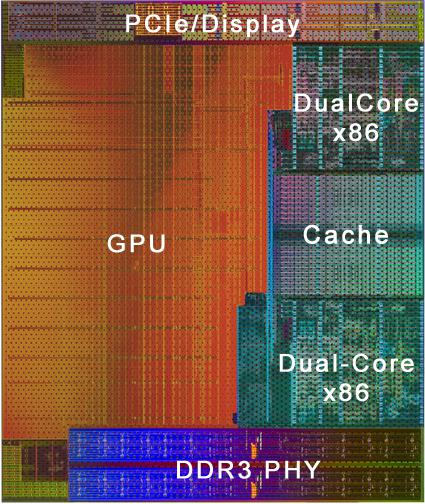
\includegraphics[scale=0.5]{img/kaveri_die}
  \caption{The AMD Kaveri quad-core CPU die layout.~\cite{web:Guru3dKaveri} Note, the DDR3 PHY unit refers to the main memory controller.}
\label{fig:kaveri-layout}
\end{figure}
% subsection amd_steamroller_architecture (end)

% section introduction_to_the_multi_core_cpu (end)



\section{Programming the multi-core CPU} % (fold)
\label{sec:programming_the_multi_core_cpu}

\subsection{Thinking parallel} % (fold)
\label{sub:thinking_parallel}
Having multiple cores available on a single chip greatly expands what is possible with the way programs are implemented and run on computers. As explained earlier in~\sectref{sub:the_multi_core_cpu}, on an $n$=core CPU, it is possible to be processing $n$ instructions concurrently at any given time.

This concurrent execution of instructions that is possible with multi-core CPUs brings the possible benefits of parallel computing, and in-turn programming, to a far greater number of computers, and thus programmers.
Before multi-core CPUs were available, parallel computing was reserved to more special-purpose computers with multiple physical CPUs (on different physical chips as opposed to a single die).

While having the hardware there to support parallel computing on the one machine, the hardware cannot magically take the all the instructions from a program and spread them out perfectly across all the cores in a system to have a fully parallelised program. This is for a number of reasons, but a lot of the time it comes back to a primitive problem being because the underlying algorithm used in a program was not designed with parallelism in mind; everything is very sequential and imperative, often because that's the way the person the algorithm was designed by learned to think about these problems.
Programming for multi-core CPUs not only requires a different style of programming, it requires the programmer to shift their mindset to think in a parallel fashion.
% subsection thinking_parallel (end)

\subsection{Example of a \vs{sequential}{parallel} algorithm} % (fold)
\label{sub:example_of_a_vs}
Take the task of doing a simple matrix multiplication on the following matrices, $matrix_A$ and $matrix_B$:

\begin{displaymath}
matrix_A =
  \begin{pmatrix}
    a_1 & b_1 & c_1 \\
    a_2 & b_2 & c_2
  \end{pmatrix}
\end{displaymath}

\begin{displaymath}
matrix_B =
  \begin{pmatrix}
    a_1 & b_1 \\
    a_2 & b_2 \\
    a_3 & b_3
  \end{pmatrix}
\end{displaymath}

If you were to do this on pen and paper, most people would probably do it following a method similar to the algorithm
shown in~\algoref{algo:matrix_mult_seq}. This method works fine for how we would naturally do it, therefore a lot of
programmers who do not know any better would perhaps write code with a similar underlying algorithm to this. That is fine,
and the computer would get the correct answer eventually after computing all $T$ the dot products, placing them where they
are meant to go in $matrix_C$, so let's say in $T$-time. Tough thinking about the problem some more, one can see that each dot product calculation
is completely independent of any other dot product calculation, only needing to share read access of values from the input
matrices. As the outcome of these dot product calculations are independent of one-another, if there were two different people,
or computers, working on the problem with $T$ dot products at the same time, we could save roughly half the calculation time by splitting the
number of dot products that need to be calculated between the two of them, letting us do the work in $T/2$-time. Now take the same problem but this time with
$n$ available computers to compute dot products. If we could split the total number of dot products, $T$, evenly between
the $n$ computers, it would be possible to get a $T/n$ speed-up in compute time. This is what is meant by computing in
parallel and what is very much possible with multi-core CPUs. A parallel version of~\algoref{algo:matrix_mult_seq} is
shown in~\algoref{algo:matrix_mult_para}.

\begin{algorithm}
\SetKwInOut{Input}{input}\SetKwInOut{Output}{output}

  \Input{Two matrices, $matrix_A$ and $matrix_B$}
  \Output{A single matrix, $matrix_C$}
  \BlankLine
  \ForEach{column $C$ in $matrix_B$}{
    \ForEach{row $R$ in $matrix_A$}{
      get dot product of $C$ and $R$
    }
  }
\caption{A sequential high-level algorithm for multiplying matrices.}
\label{algo:matrix_mult_seq}
\end{algorithm}

\begin{algorithm}
\SetKwInOut{Input}{input}\SetKwInOut{Output}{output}
\SetKwProg{Fn}{Function}{is}{end}
\SetKwFunction{FnWorker}{calculateDotProducts}

  \Input{Two matrices, $matrix_A$ and $matrix_B$, pool of workers, $workerPool$}
  \Output{A single matrix, $matrix_C$}
  \BlankLine
  $numWorkers = getNumAvailableWorkers()$

  $numDotProducts = getNumDotProducts()$

  \BlankLine
  \ForEach{worker $W$ in $workerPool$}{
    $dotProducts[] = getNewDotProducts(numDotProducts/numWorkers)$

    call calculateDotProducts(dotProducts[]) on $W$
  }

  \BlankLine
  \BlankLine
  \Fn{\FnWorker{dotProductCalculations[]}}{
    \ForEach{dot product calculation $DP$ in $dotProductCalculations$}{
      perform $DP$
    }
  }
\caption{A parallel high-level algorithm for multiplying matrices.}
\label{algo:matrix_mult_para}
\end{algorithm}

Something of note is that there are limits to the benefits the parallel algorithm has over the sequential algorithm.
If the number of workers is greater than the number of dot product calculations that need to be performed, there
are going to be some workers that have nothing to do. This means that any increase in the number of workers after this point
is meaningless in-terms of making computations faster.

Furthermore, if there is only a single worker, then the computations of dot products are essentially all going to be performed
sequentially, just as in the sequential algorithm.
% subsection example_of_a_vs (end)

\subsection{Models for enabling of parallel and concurrent programming} % (fold)
\label{sub:enablers_for_programming_in_parallel}
The idea and theory behind the benefits of programming in parallel is all well and good, although there need to be some
underlying programming models that to enable these parallel algorithms to be implemented.

\subsubsection{Multiple threads of execution} % (fold)
\label{ssub:threads_execution}
One notable, and very widely
used, method to allow concurrent and, in-turn, parallel programming is through the use of threads. Threads are now a core
underlying part of all widely-used modern operating systems. Threads allow the programmer to specify multiple threads
of execution to run concurrent to one another to perform some particular logic. At a lower-level of the operating system,
beyond the area of the application programmer's concern, the kernel handles the scheduling of all these different concurrent threads
to be run on different cores if possible. Running the threads of different cores means that they can be run truly in parallel
rather than concurrently sharing processor time on a single core. There are numerous APIs available to applications programmers
in different programming languages
allowing them to implement threads in their applications allowing the possibility of parallel programs on multi-core systems.
Some popular APIs include:
\begin{itemize}
  \item POSIX Threads (commonly referred to as ``Pthreads'')
  \item Java's ``java.util.concurrent'' package
  \item .NET's Thread Pool API
\end{itemize}
% subsubsection subsubsection_name (end)

\subsubsection{Message passing between processes} % (fold)
\label{ssub:message_passing_between_processes}
The concept of message passing is simply that; the passing of messages between processes. Message passing as a concept is
not exactly a model to allow parallel programming, although used indirectly, it makes concurrent and parallel programming
possible. If there are multiple processes running on a multi-core machine, perhaps some processes on different cores, by
operating system design, they are generally completely isolated from one another in terms of instructions and data. Message
passing lets these independent processes communicate and thus similar concurrency that we've seen in threads can be achieved.
Another important topic related to parallel computing in general, although not directly to multi-core CPUs, is that a
properly configured message passing system can allow parallel distributed computing, for example over networks, and abstract
it in such a way that the programmer need not be concerned about the host computer for particular processes. One notable
message passing system that does exactly this is Message Passing Interface (MPI), which has become somewhat of an unofficial
standard for message passing.
% subsubsection message_passing_between_processes (end)

% subsection enablers_for_programming_in_parallel (end)

% section programming_the_multi_core_cpu (end)



\section{Introduction to the GPU} % (fold)
\label{sec:introduction_to_the_gpu}

\subsection{The graphics processing unit} % (fold)
\label{sub:the_graphics_processing_unit}
The graphics processing unit --- hereby referred to as the GPU --- is a specialised processor designed to facilitate the
output of images and computer graphics through means of rapidly manipulating memory~\cite{web:WikiGPU}. Traditionally,
GPUs have been used since the early 1980s to perform various computer graphics operations independent of the CPU, allowing
the CPU to focus on traditional CPU operations, as explained in~\sectref{sec:introduction_to_the_multi_core_cpu}. These
computer graphics operations originally consisted of relatively simple operations such as the drawing of lines, filling
specified areas in a framebuffer. Since then, GPUs have been adapted for use with much more intensive tasks such as
the rendering of three-dimensional graphics in movies, or even the realtime calculating and drawing of three-dimensional
video game graphics. While far more processing intensive, these tasks may be using many sequences of the same underlying
graphics operations they always have done. While certainly being impressive, facilitating the output of fancy graphics is
not the only thing GPUs are used for. As we will soon see, through an analysis of their underlying architecture, GPUs
offer very impressive power and possibilities in the field parallel computing that simply cannot, at present, be found
in offerings from CPUs.

Note that there is an important difference between the terms ``GPU'' and ``graphics card'', which can often be found
being used interchangebly in places such as news articles, marketing information, and online message boards. A GPU refers
to the actual graphics processing chip, which are often present on all graphics cards. Although a computer may also have
a GPU if it does not have a discrete graphics card. As was noted in~\sectref{sub:multi_core_cpu_architecture}, GPUs are
often present on the same chip as the CPU in many modern CPU offerings from companies such as AMD or Intel. This is
often referred to as ``integrated graphics'' (as opposed to ``discrete graphics'').
% subsection the_graphics_processing_unit (end)

\subsection{GPU architecture} % (fold)
\label{sub:gpu_architecture}
The general GPU architecture differs quite substantially from a general CPU architecture, what was seen
in~\sectref{sub:multi_core_cpu_architecture}. One of the most obvious differences is the number of processing cores
that are available to both. As we have seen in CPUs, they were originally designed as single-core pieces of hardware,
before it became more common to sell them with multiple cores. Although as the number of cores that comes standard on
CPUs seems to be increasing as the years go on, most modern consumer CPUs nowdays have four or eight cores. When we
look at GPUs, most common modern consumer GPUs ship with thousands of cores on the single chip (see~\figref{fig:gpu-vs-cpu}).
Of course, these cores are considerably different to those cores found on CPU chips.

\begin{figure}[ht]
  \centering
  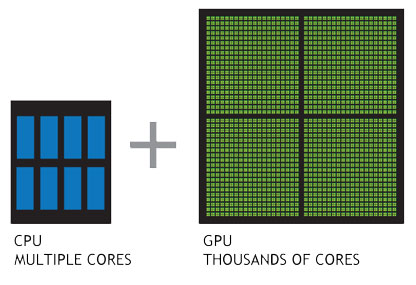
\includegraphics[scale=0.5]{img/cpu-and-gpu}
  \caption{GPUs contain large arrays of thousands of cores, allowing them to partition workloads amongst the cores,
  having more potential to be parallel programmed. CPUs contain a far smaller amount of more specialised cores, more
  optised for performing sequential tasks.~\cite{web:NvidiaCPUvsGPU}}
\label{fig:gpu-vs-cpu}
\end{figure}

CPU cores are more optimised for sequential serial processing of instructions, while GPU cores are a lot smaller, have
far less complicated circuitry and are designed to handle more simple tasks in a simultaneous fashion~\cite{web:NvidiaGPUComputing}.

Some very recent and widely used evolutions in modern consumer GPU architectures would have to Nvidia's very recent Maxwell
microarchitecture and AMD's Sea Island microarchitecture.

Nvidia's Maxwell architecture is Nvidia's successor for their widely used Kepler architecture. It is currently, as of
mid 2014, being used in Nvidia's GeForce 700 Series consumer GPUs, and while not offering too much new functionality
from the predecessor architecture, Kepler, it has a large focus on power savings and increasing the performance given
per watt consumed~\cite{whitepaper:NvidiaMaxwell}.

AMD's Sea Islands architecture is one of AMD's newest implementations of their ``Graphics Core Next'' (GCN) GPU
architecture. The GCN architecture has been in use as the basis of AMD GPUs since late 2011, hence a lot of the information
presented here on the Sea Islands family of GPUs is also relevant to other GCN GPUs~\cite{web:AnandGCNPreview}. Sea Islands,
specifically, was used by AMD for their Radeon HD 8000 consumer series of GPUs.

\subsubsection{Nvidia's Maxwell architecture} % (fold)
\label{ssub:nvidia_maxwell_architecture}
As a specific example of a Maxwell implementation, we can have a look at Nvidia's relatively new GM107 GPU which ships
with Nvidia's new GeForce GTX 750 Ti graphics card, commercially available.

The way the GPU is laid out is
by having a single Graphics Processing Cluster (GPC), which is essentially a cluster of all the cores available within the GPU.\@
Inside the GPC, the cores are separated into five groups called Maxwell Streaming Multiprocessors (SMMs), each of which have
are arbitrated by the GPC's Raster Engine. The GPC then has its own 2048 KB L2 cache (which is shared between all the SMMs
contained inside the GPC). Of course, the GPU needs access to larger memory levels which is facilitated through the use of dual
64-bit memory controllers~\cite{whitepaper:NvidiaMaxwell}. This can all be seen from the block diagram shown in~\figref{fig:maxwell-gm107}.

\begin{figure}[ht]
  \centering
  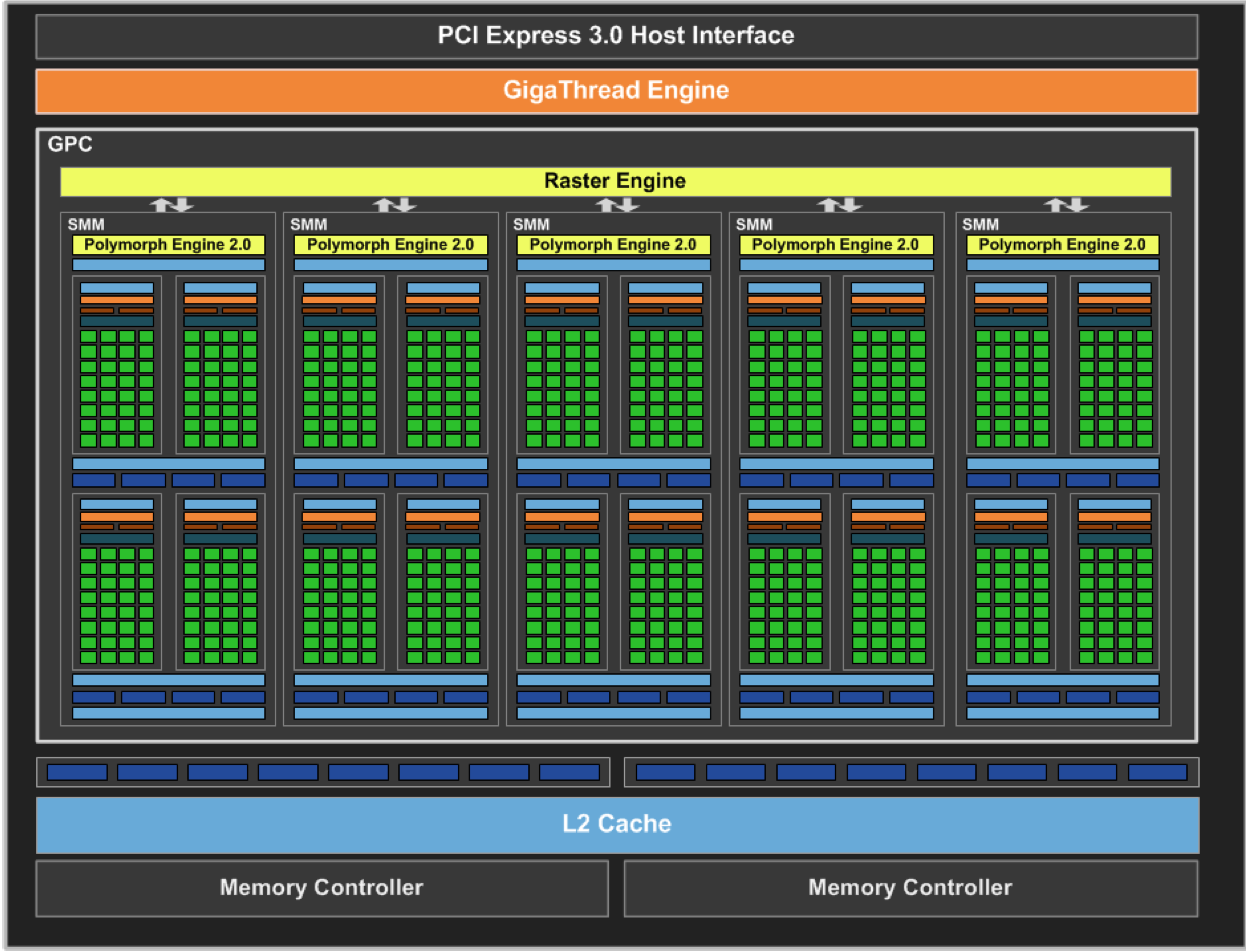
\includegraphics[scale=0.3]{img/maxwell-chip}
  \caption{Nvidia's Maxwell based GM107 GPU chip layout.~\cite{whitepaper:NvidiaMaxwell}}
\label{fig:maxwell-gm107}
\end{figure}

Going down another level into the Maxwell Streaming Multiprocessors, each SMM has a large number of cores split up into
four main groups, along with a large instruction cache, and two L1 caches, each of which is shared by two of the four
distinct groups of cores. Each of these groups of cores has its own instruction buffer, warp scheduler, dispatch units and a large
register file. Essentially what these components do is facilitate the scheduling and dispatching of instructions from the
larger instruction cache to specific cores to be processed. Another component of note in these SMMs is the presence of
64 KB block of shared memory. This shared memory is shared between each of the distinct core groups, offering even more
possibility of parallel processing~\cite{whitepaper:NvidiaMaxwell}. The specifics of an SMM model are depicted in~\figref{fig:maxwell-smm}.

\begin{figure}[ht]
  \centering
  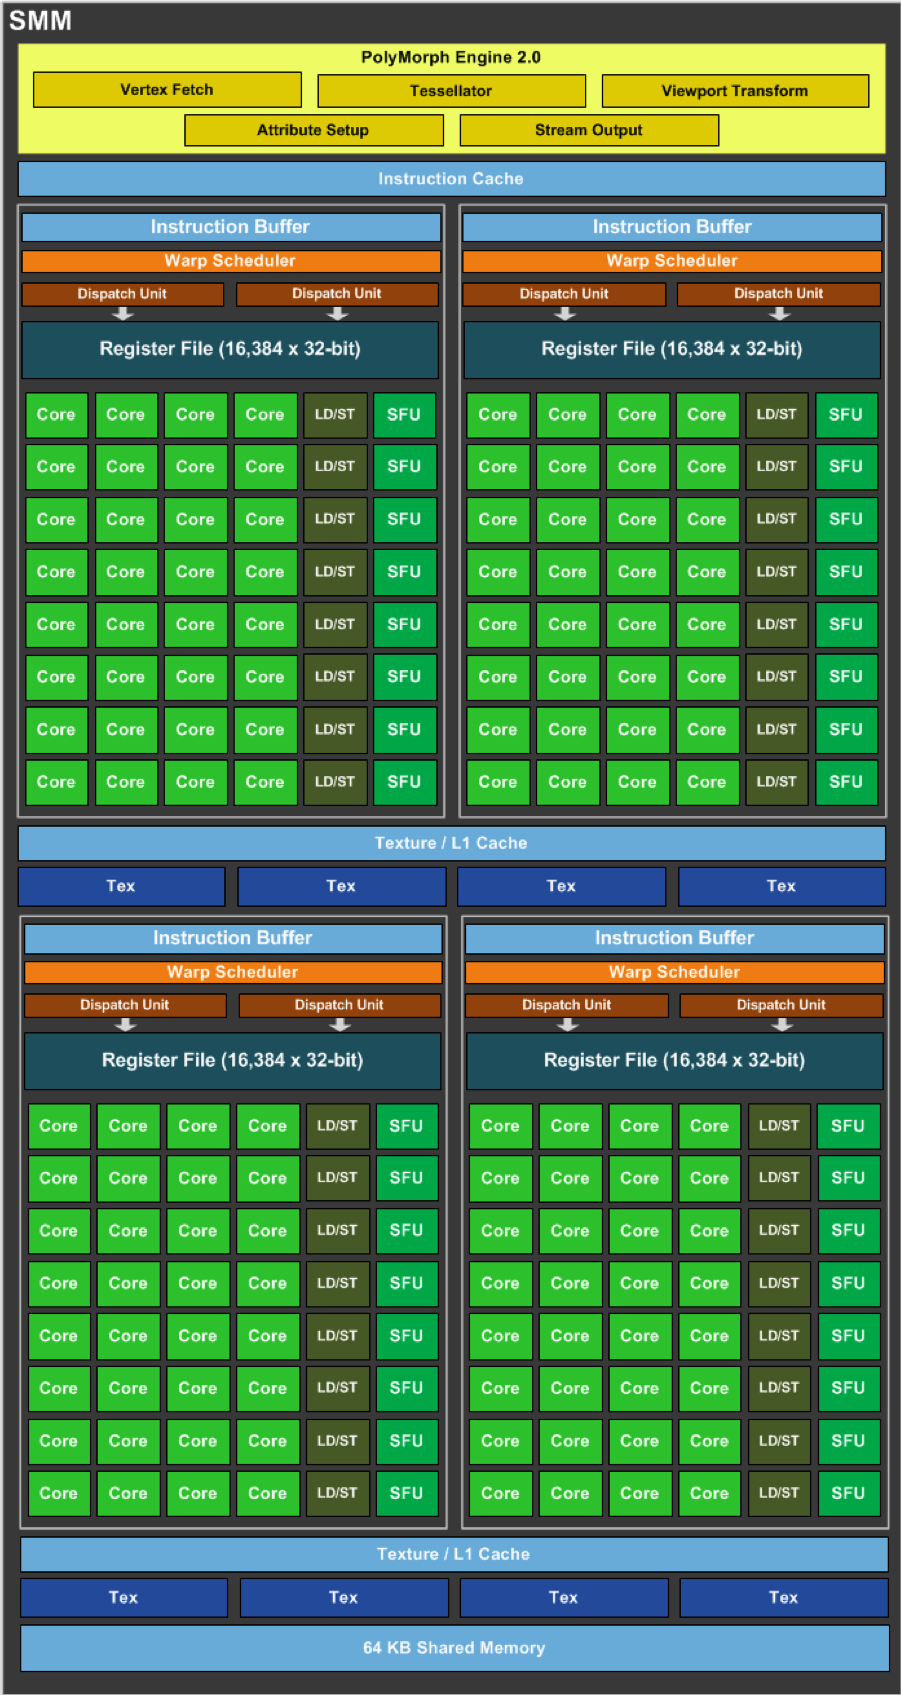
\includegraphics[scale=0.25]{img/maxwell-smm}
  \caption{Nvidia's Maxwell Streaming Multiprocessor layout.~\cite{whitepaper:NvidiaMaxwell}}
\label{fig:maxwell-smm}
\end{figure}

Something of note is that the GM107 alone houses 640 cores, all of which can be used to perform different operations
simultaneously. As discussed in~\sectref{sec:programming_the_multi_core_cpu}, with a highly parallelised algorithm or
program, the sheer number of cores accessible here is really going to become an advantage over the same task being performed
on far less parallel-optimised multi-core CPU hardware.
% subsubsection nvidia_maxwell_architecture (end)

\subsubsection{AMD's Sea Islands/Graphics Core Next architecture} % (fold)
\label{ssub:amd_s_sea_islands_graphics_core_next_architecture}
Rather than looking at a specific Sea Islands implementation, we will look at a more generic overview of what is offered
by any Sea Islands based GPU.

The way the GPU architecture is laid out is by assembling all of the individual cores into a large array known as the
Data-Parallel Processor (DPP) array. The DPP array can be thought of as being akin to the Nvidia Maxwell's group of SMMs,
and is essentially where the main processing power of the GPU lies. Instructions are fed into the DPP array through the
use of a Command Processor in conjunction with a dispatcher component. Shared between the entire DPP array is a bus known
as the CrossBar which facilitates access to the different L2 caches.
The L2 caches are then
connected to a single memory controller allowing direct memory access back to larger memory devices~\cite{reference:AMDSeaIslandsISA}.
This can all be visualised in~\figref{fig:sea-islands-chip}, although it is slightly more confusing than Nvidia's Maxwell
chip layout.

\begin{figure}[ht]
  \centering
  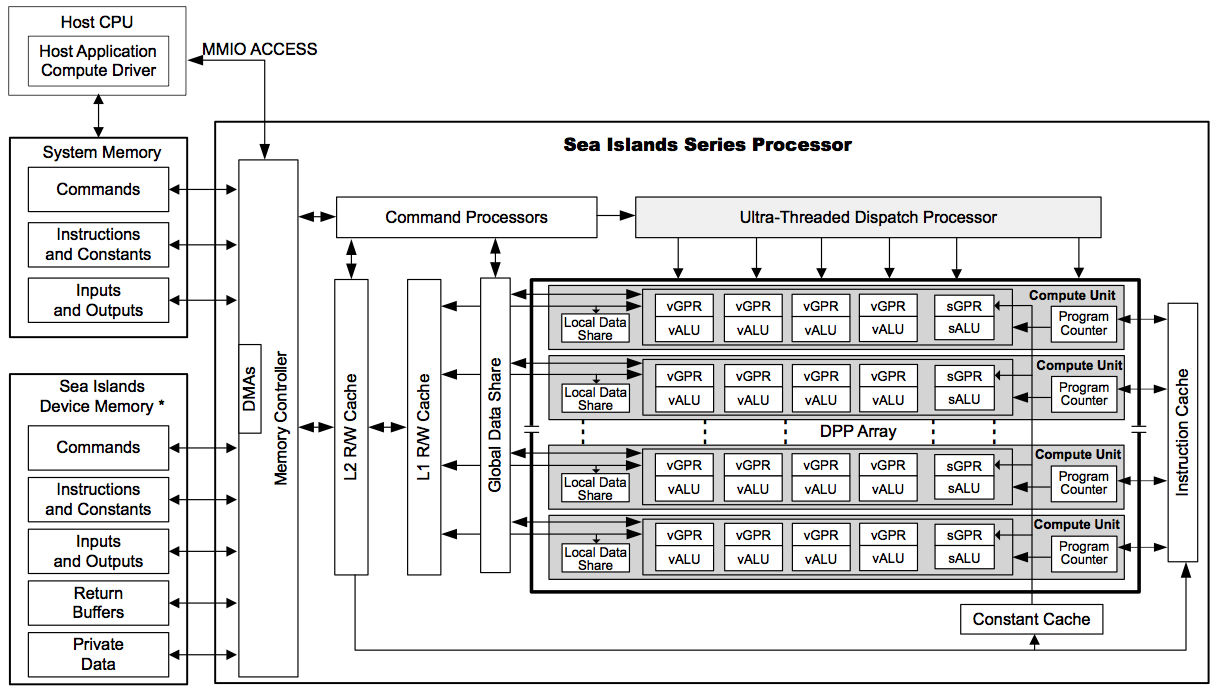
\includegraphics[scale=0.3]{img/sea-islands-chip}
  \caption{AMD's Sea Islands GPU chip layout.~\cite{reference:AMDSeaIslandsISA}}
\label{fig:sea-islands-chip}
\end{figure}

Going deeper into the Data-Parallel Processor, each DPP has $n$ number of single instruction, multiple data components
(SIMDs), each of which contains 64 cores (although here they are known simply as ``processors''). Each of these cores has
its own general purpose data register and access to the SIMD's 32 KB of shared memory. On top of this per-SIMD shared memory,
there is also the 64 KB Global Data Share (GDS), which is shared between all SIMDs. The GDS also has access to each
of the SIMD's L1 texture caches~\cite{reference:AMDSeaIslandsISA}. This can all be seen in~\figref{fig:sea-islands-sm}.

\begin{figure}[ht]
  \centering
  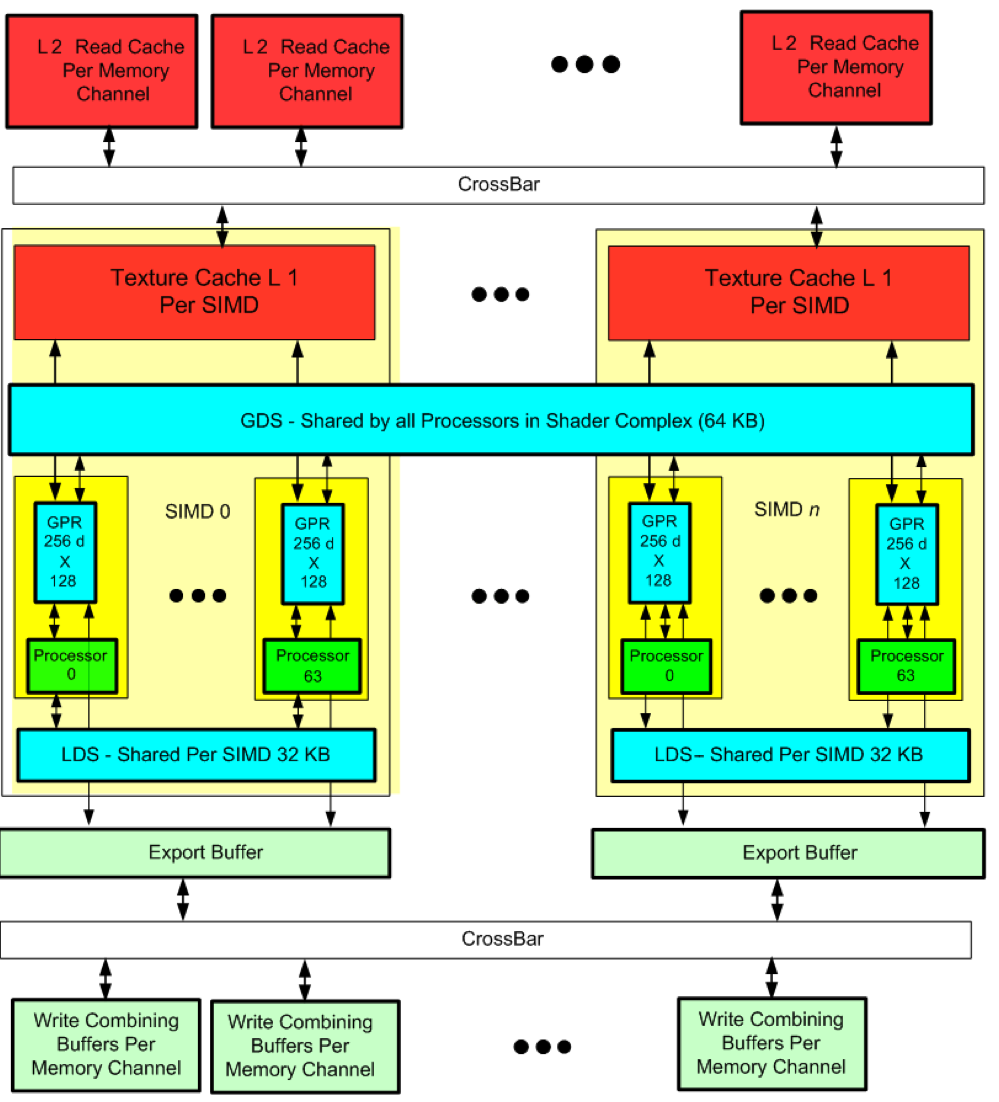
\includegraphics[scale=0.3]{img/sea-islands-sm}
  \caption{AMD's Sea Islands GPU Stream Processor layout.~\cite{reference:AMDSeaIslandsISA}}
\label{fig:sea-islands-sm}
\end{figure}

% subsubsection amd_s_sea_islands_graphics_core_next_architecture (end)

\subsubsection{Distinctions between the GPU architectures and CPU architectures} % (fold)
\label{ssub:distinctions_between_the_gpu_architectures_and_cpu_architectures}
While both GPU architectures may have differently named components, we can see a very similar underlying concepts between
the two that  are quite different to the way the previously analysed CPU architectures are designed. Most notable, as
previously mentioned, is the greatly increased number of distinct cores, or simply elements of processing in general.
Because of this emphasis on a greater number of processing cores in the GPUs, we also see an emphasis on architectural
components such as shared memory between the cores, grouping of cores into arrays and different super-collections of cores.
Each of these collections also have some form of shared memory. There also was, of course, an emphasis on components
concerned with the dispatch and scheduling of instructions. Without this type of organisation in the underlying architecture,
the hardware would have a very hard time facilitating such largely parallel use-cases.
% subsubsection distinctions_between_the_gpu_architectures_and_cpu_architectures (end)

% subsection gpu_architecture (end)

% section introduction_to_the_gpu (end)


\section{Differences in programming the GPU} % (fold)
\label{sec:differences_in_programming_the_gpu}

\subsection{Why the CPU has not been abandoned for the GPU} % (fold)
\label{sub:why_programs_aren_t_written_just_for_gpus_rather_than_cpus}
After seeing the massively parallel processing power made possible through the GPU, one may naturally ask the question:
``Why don't we just target our programs toward the GPU to take advantage of that parallelism?''. As we have already seen,
the CPU and the GPU have very different architectures and are thus optimised for completely different tasks; the GPU
should not just be thought of as a substitute for the CPU.

Furthermore, there is the problem that not every task can be parallelised; just like in real-life, there will be times when
no work can proceed until another piece of work that the current one depends on has first been completed. This is often encountered
in programs that have to wait for data to be received. For example, going back to the matrix multiplication example in
~\sectref{sub:example_of_a_vs}, the entire first part of the algorithm is done serially and there will be no performance gain
over the sequential algorithm until that serial part is first taken care of, thus setting up the parallel part to be run.

Additionally, less related to the actual hardware architecture and underlying algorithms of software, there is also the
unfortunate aspect that programming a GPU is significantly different than programming a CPU, and as arguably fewer programmers
have had experience actually programming a GPU, this poses a barrier to adoption of more ``GPU-accelerated'' programs.
The way of programming a GPU involves new languages, extensions of existing languages, and even completely new programming
paradigms and ways of thinking about code. The reason for this difference does relate back to the architectural differences
in GPUs and CPUs in the way that these different ways of programming GPUs directly relate expressing routines in parallel
that existing languages and programming paradigms simply did not facilitate, or make it too unnatural. This leads on to
the topic of general purpose computing on GPUs (GPGPU).

% subsection why_programs_aren_t_written_just_for_gpus_rather_than_cpus (end)

\subsection{General purpose computing on GPUs, or GPGPU} % (fold)
\label{sub:general_purpose_computing_on_gpus_or_gpgpu}
While GPUs were originally designed with computer graphics functionality in mind, GPUs are now often used for general
purpose computing tasks that were traditionally left for CPUs~\cite{web:WikiGPGPU}. Ideally these tasks would involve
large parallelism to get the most benefit out of using a GPU, else they would be better left to be serially processed
on a CPU. GPUs can essentially be thought of as large scale stream processors, meaning that they are ideal for parallel
processing involving the execution of a single function over many different elements of data in a set of data (the stream).
The perfect application for GPGPU is then those applications which involve large streams of data with minimal to no
dependencies between those elements of data~\cite{Buck:2004:BGS:1015706.1015800}. To facilitate GPGPU, high-level languages
and frameworks have been developed. The arguably most popular modern offerings to facilitate GPGPU are the open-source
Open Computing Language --- more commonly referred to as ``OpenCL'' --- and the Nvidia's proprietary Compute Unified
Device Architecture --- more commonly referred to as just ``CUDA''. CUDA only supports Nvidia GPUs~\cite{web:NvidiaCUDACompat},
although is still reasonably popular, while OpenCL supports a far larger range of GPUs from different vendors, including
AMD, Nvidia, Intel and IBM~\cite{web:KhronosOpenCLCompat}.


\subsubsection{Overview of OpenCL} % (fold)
\label{ssub:overview_of_opencl}
OpenCL, as previously stated, is an open-source framework for facilitating GPGPU. While facilitating GPGPU, OpenCL's bigger
aim to make heterogeneous computing more of a reality~\cite{slides:KhronosOpenCLOverview}. That is, seamlessly integrating general CPU operation with the operation
of GPUs in the overall system. For example, passing all serial operations straight to the CPU which then sets up all parallel
operations to run on the GPU would be ideal heterogeneous computing in which each piece of hardware performs the task
that it is optimised for.

OpenCL defines its language as a subset of ISO C99, with extensions. A function written in this language is referred
to by the somewhat confusing name of a ``kernel''. While it may look a lot like standard C99 code, the way OpenCL executes
its programs differs considerably, and can be seen as being very intimidating in its difference.

The first requirement of execution of an OpenCL program is a single or multiple OpenCL compatible devices. Once the devices
are found on a host, programs need to be loaded to execute on the given devices. Note that programs here just refers to
a collection of kernels. From these programs, specific kernels need to be explicitly specified to execute and supplied to
a command queue to await execution. Of course, data to execute the kernels on needs to be loaded to the particular devices
that the kernels will be executed on in the form of memory objects. After the kernel is done executing on the given data,
the result needs to be sent back from the device to the host~\cite{slides:KhronosOpenCLOverview}. This long-winded sequence of execution can be visualised
in~\figref{fig:opencl-execution}.

\begin{figure}[ht]
  \centering
  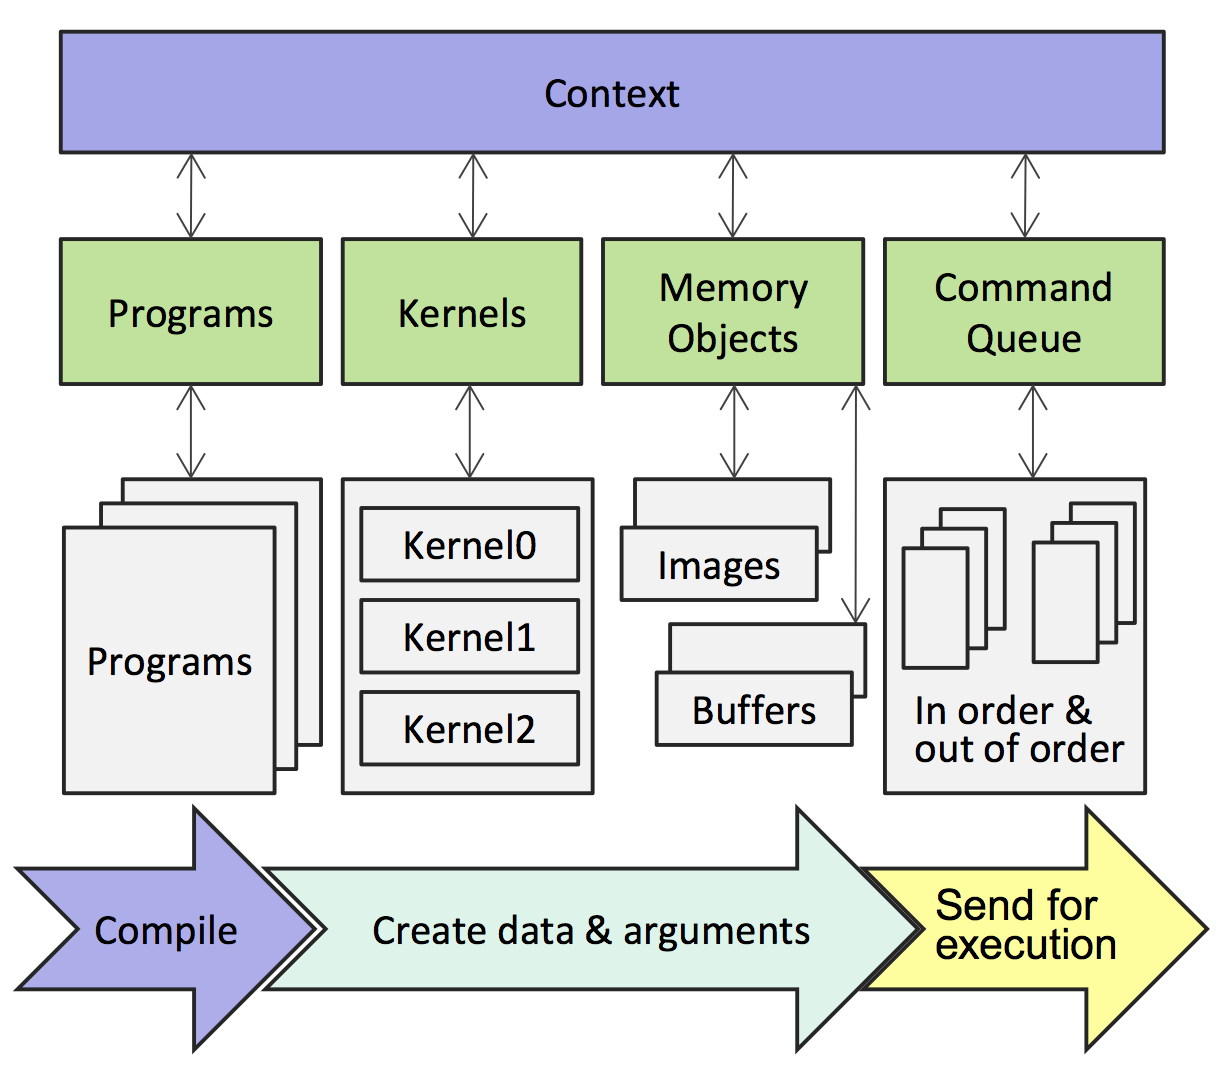
\includegraphics[scale=0.5]{img/opencl-execution}
  \caption{The long sequence of execution provided by OpenCL. Note that most of these steps need to be explicitly stated
  in the code.~\cite{slides:KhronosOpenCLOverview}}
\label{fig:opencl-execution}
\end{figure}

Given the complexity of execution and the difference in paradigm and style of thinking needed, OpenCL kernels should be
written with this in mind, rather than being constrained to work with a particular predicted element of data.
A simple example demonstrating a change is shown in~\figref{fig:opencl-code}.

\begin{figure}[ht]
  \centering
  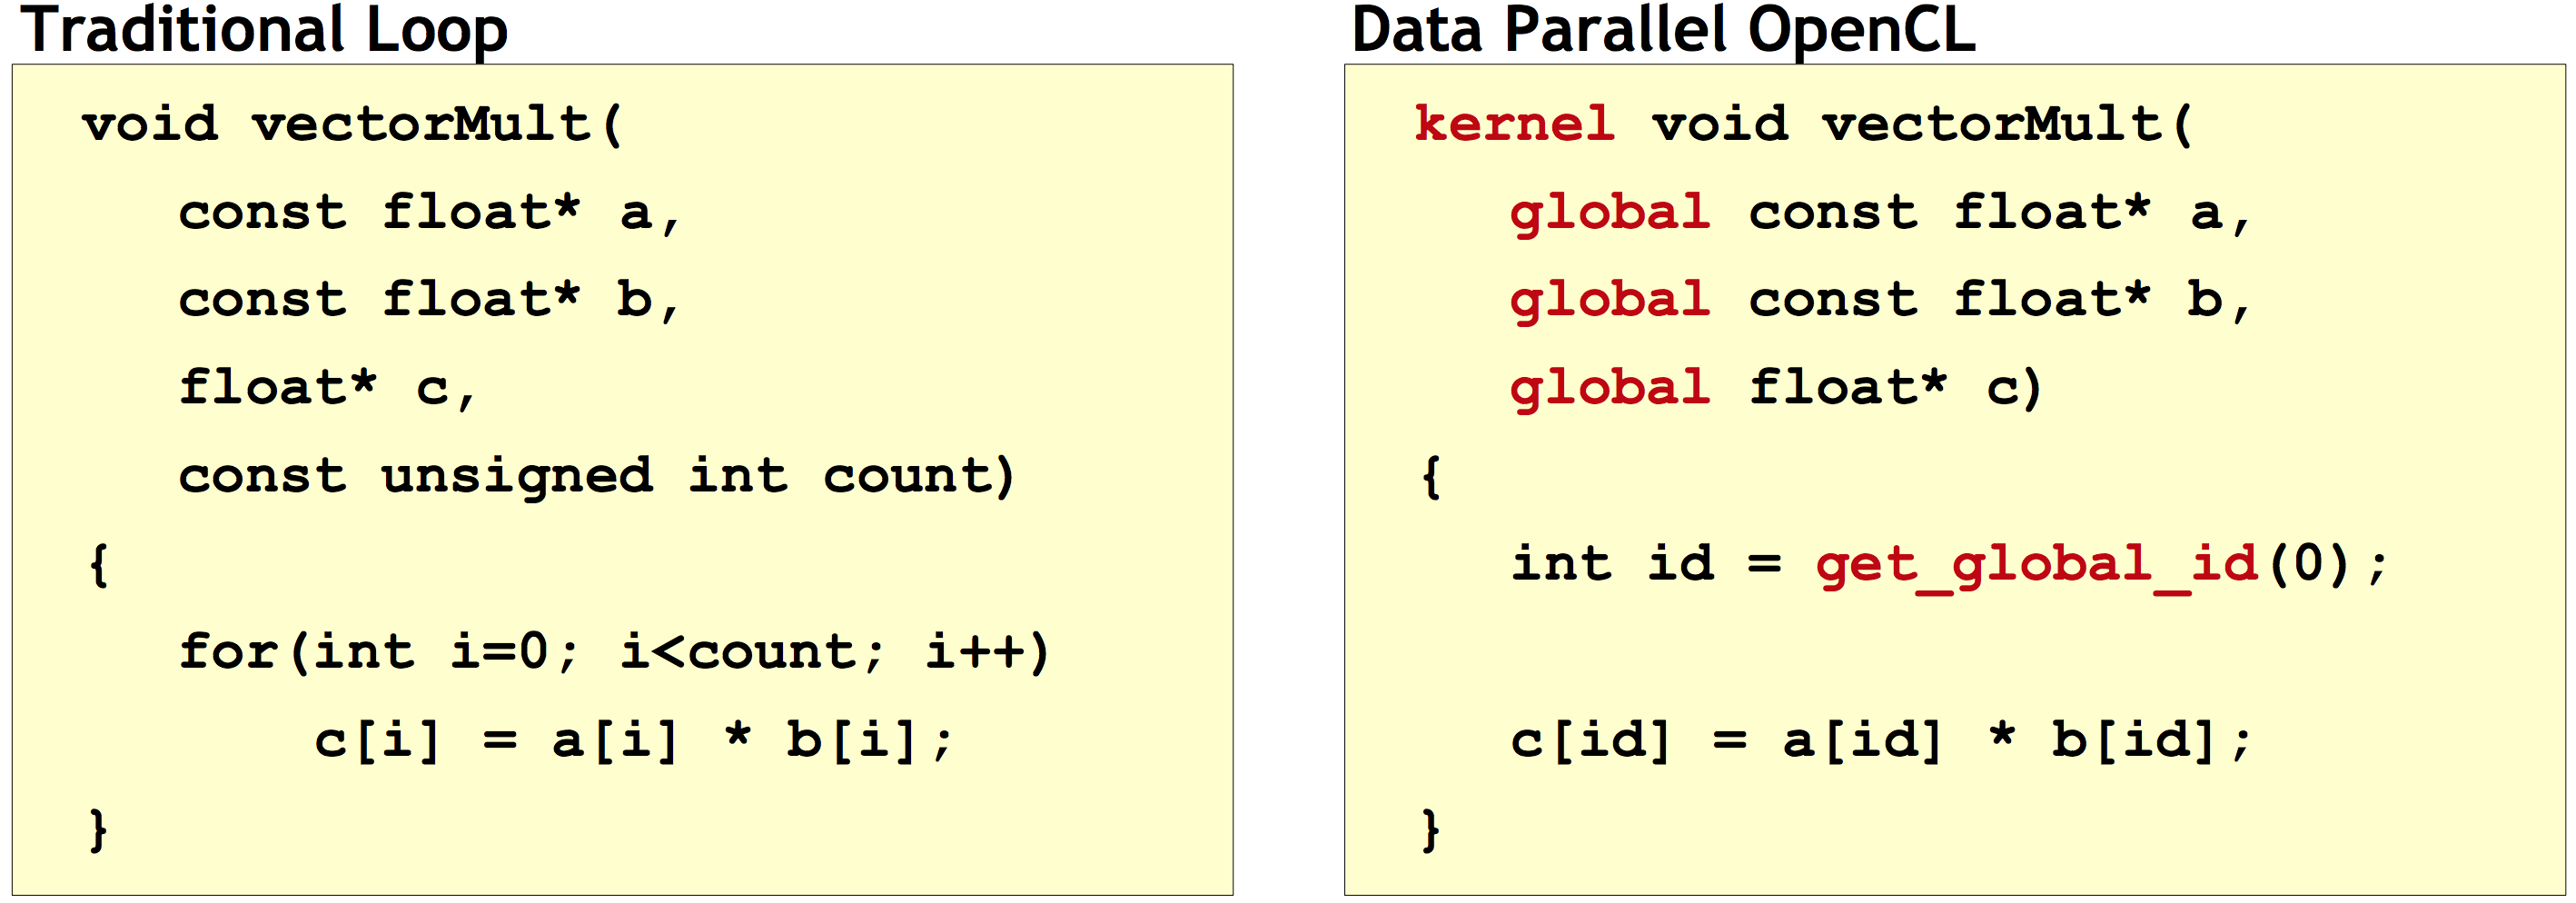
\includegraphics[scale=0.2]{img/opencl_code}
  \caption{The big idea behind OpenCL; programming in $n$-dimensions rather than the, arguably, more ``traditional''
  $1$-dimension imperative paradigm of programming.~\cite{slides:KhronosOpenCLOverview}}
\label{fig:opencl-code}
\end{figure}

Note that OpenCL also specifies its own logical memory hierarchy that attempts to convey a generic physical hierarchy.
A general overview of OpenCL's logical memory hierarchy can be summarised as follows:
Each work-item (execution of a kernel) has its own private memory. Workgroups as a whole have their own shared
local memory. All workgroups have access to an unsynchronised global/constant memory which can be filled from the main
system memory. Note that memory management between hierarchy levels must be explicitly stated in the
kernels~\cite{slides:KhronosOpenCLOverview}. The OpenCL hierarchical memory model is depicted in~\figref{fig:opencl-mem-model}.

\begin{figure}[ht]
  \centering
  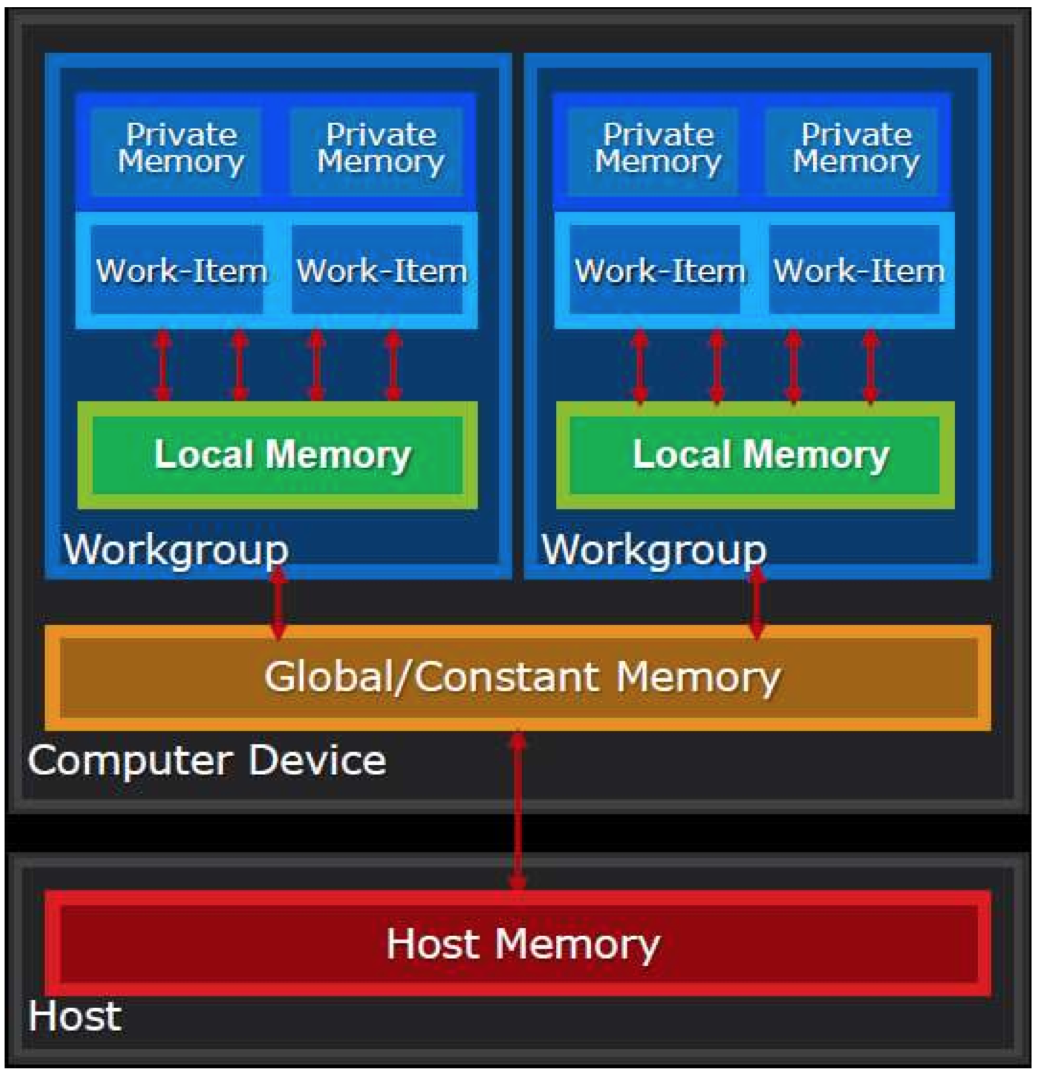
\includegraphics[scale=0.5]{img/opencl-mem-model}
  \caption{OpenCL's memory hierarchy.~\cite{slides:KhronosOpenCLOverview}}
\label{fig:opencl-mem-model}
\end{figure}
% subsubsection overview_of_opencl (end)

\subsubsection{Overview of CUDA} % (fold)
\label{ssub:overview_of_cuda}
Nvidia's CUDA is a proprietary framework that facilitates the use of compatible Nvidia GPUs in general purpose computing.
Like OpenCL, it attempts very much to facilitate heterogeneous computing using GPUs and CPUs together. Much like OpenCL,
CUDA has the concept of kernels being functions that are called by the host to execute on CUDA compatible devices. Kernels
are, again, written in a subset of C with restrictions regarding memory access, and with language extensions~\cite{slides:KhronosOpenCLOverview}.

Where CUDA tries to differentiate itself from OpenCL is shown in its emphasis on how kernels are executed using its own
concept of threads. These threads conceptually reflect traditional threads, as previously looked at in~\sectref{ssub:threads_execution}.
Rather than a kernel being executed by a specific GPU core, CUDA splits a kernel into many different threads, even thousands,
which are then grouped in ``blocks''. Blocks are then grouped into a ``grid'' which roughly reflects the logical architecture
of the GPU. This whole kernel is then executed by the GPU as a grid of blocks of threads. This is the reason why Nvidia
uses the term ``CUDA core'' to refer to their GPU cores; because the actual GPU cores physically represent a unit of
execution in CUDA; the CUDA thread~\cite{slides:KhronosOpenCLOverview}.

To divide the concept up some more, basically the individual threads are a logical representation of a physical core. Each
block of threads is a logical representation of a streaming multiprocessor (as looked at in~\sectref{ssub:nvidia_maxwell_architecture} as SMMs).
Finally, each grid is a logical representation of an entire GPU. Hence the CUDA framework allows an almost one-to-one
logical matching with the physical device on which it is executing~\cite{slides:KhronosOpenCLOverview}. A visual depiction of this can be seen in~\figref{fig:cuda-mapping}.

\begin{figure}[ht]
  \centering
  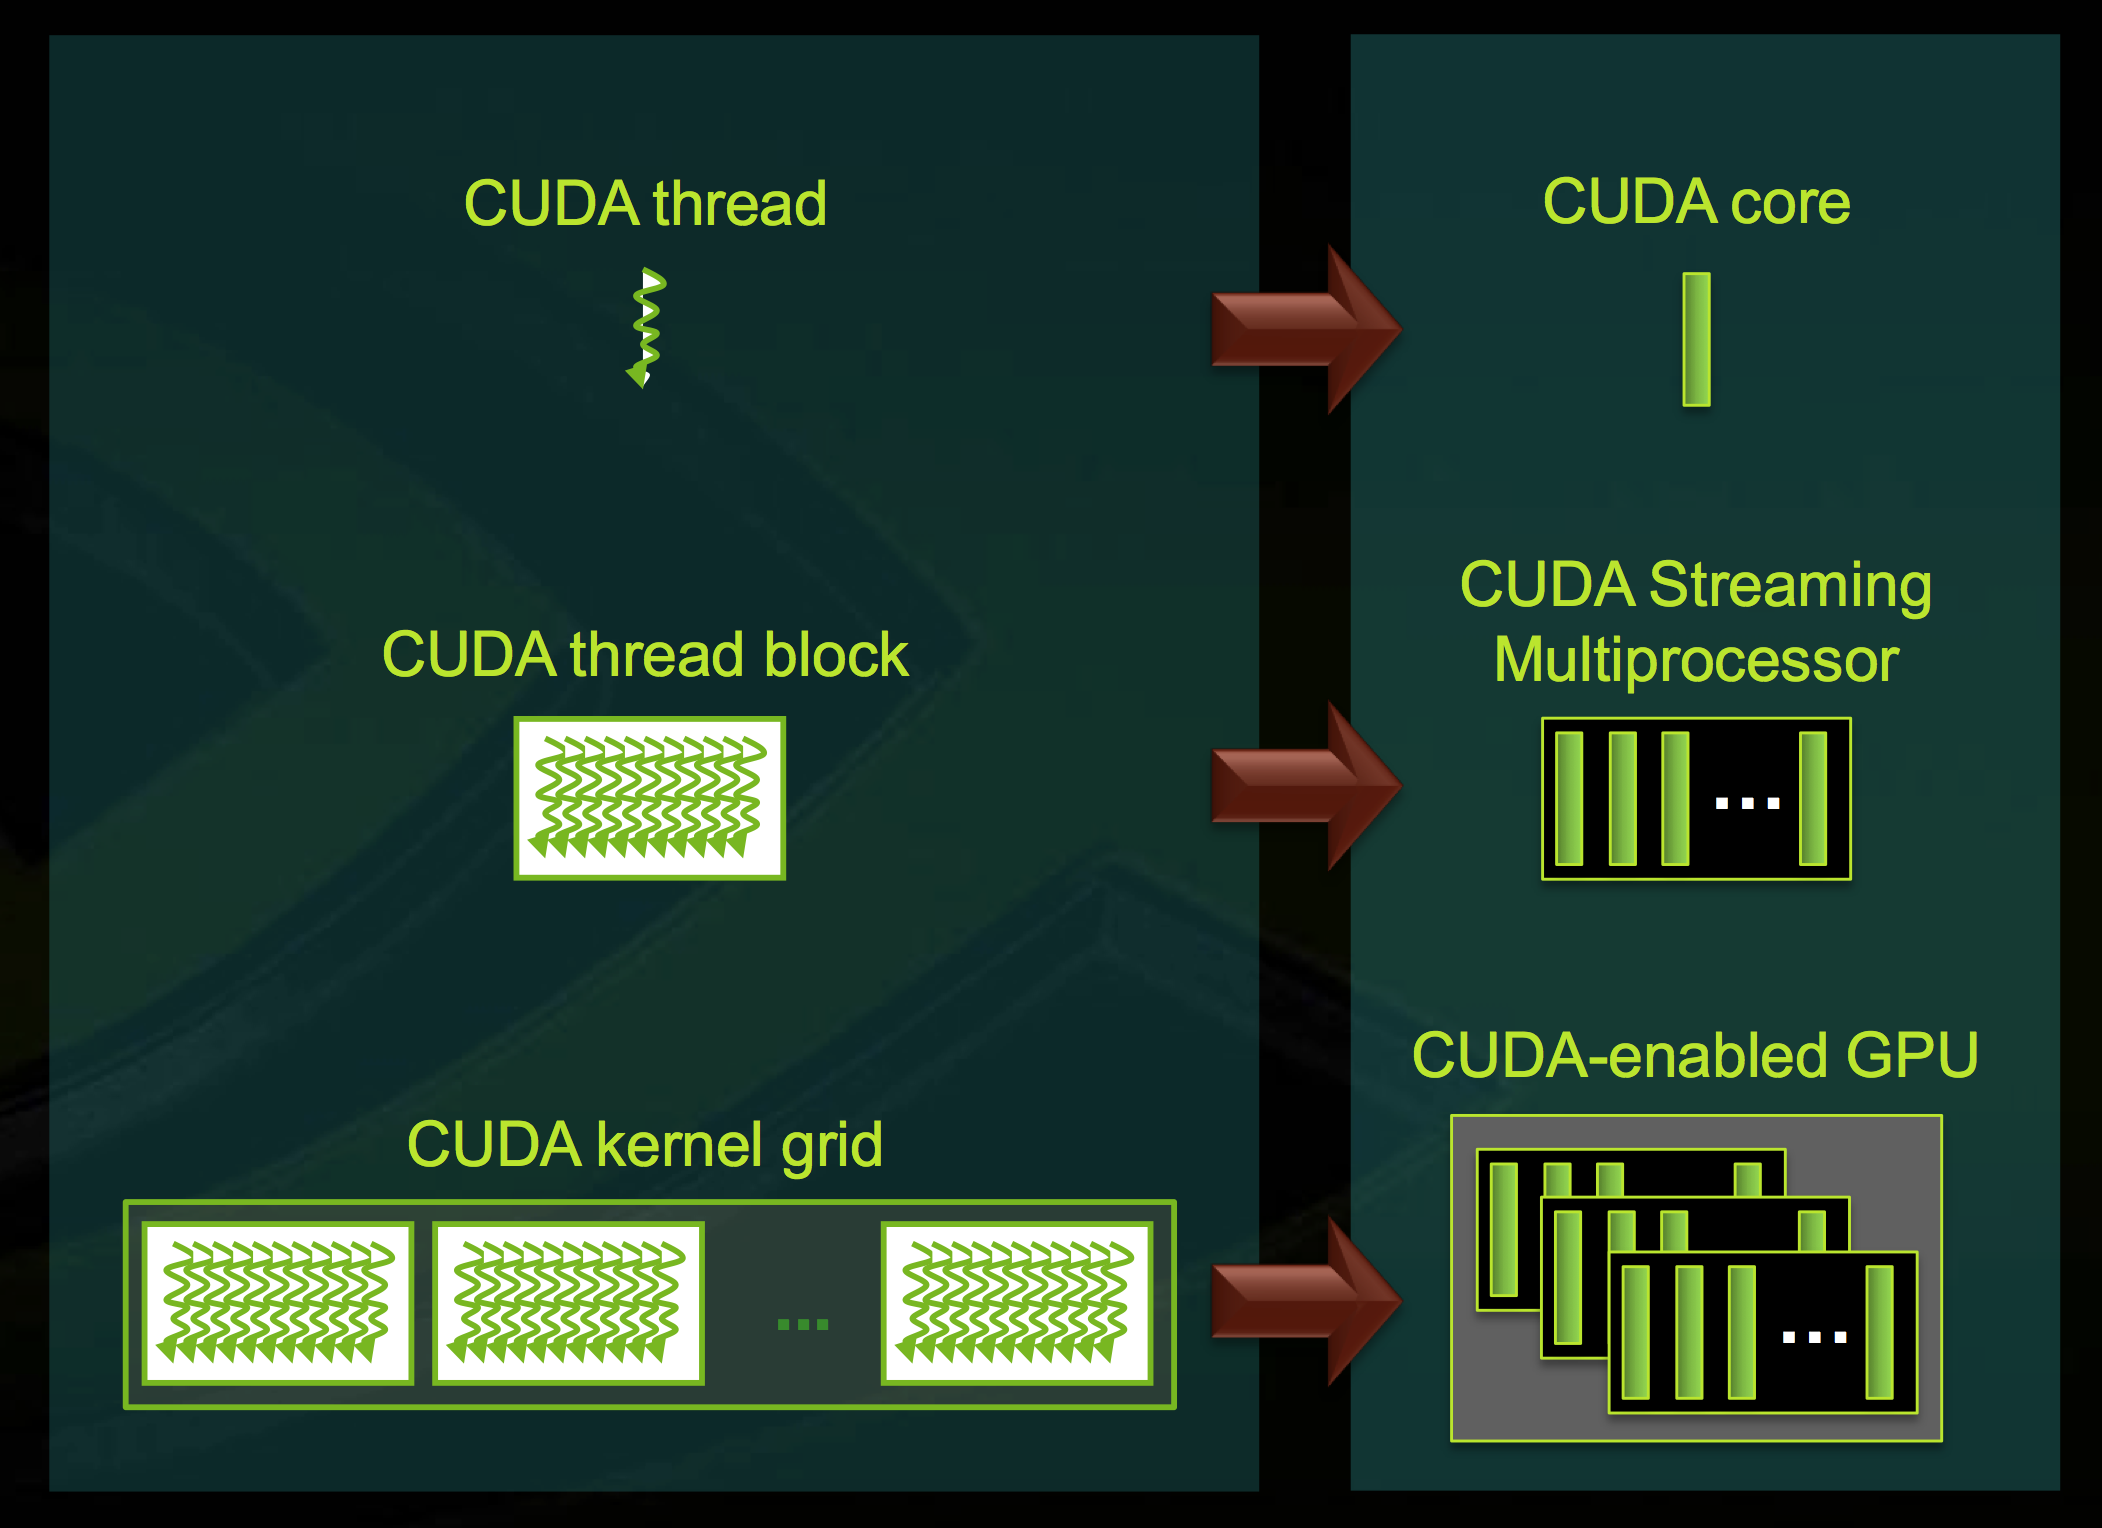
\includegraphics[scale=0.2]{img/cuda-mapping}
  \caption{The logical CUDA framework mapping to a physical CUDA-compatible GPU.~\cite{slides:KhronosOpenCLOverview}}
\label{fig:cuda-mapping}
\end{figure}

Much like the physical layout of the SMMs, CUDA blocks afford cooperation with each other and as well as being able to be
executed in parallel, they have the important the ability of being able to be easily executed in sequence and synchronised
with each other, as is often important, even in mostly parallel processing.

Much like OpenCL, CUDA specifies its own logical memory hierarchy which integrates into its logical architecture of
threads, blocks of threads, and grids. The memory hierarchy can be viewed in more detail in~\figref{fig:cuda-mem}.

\begin{figure}[ht]
  \centering
  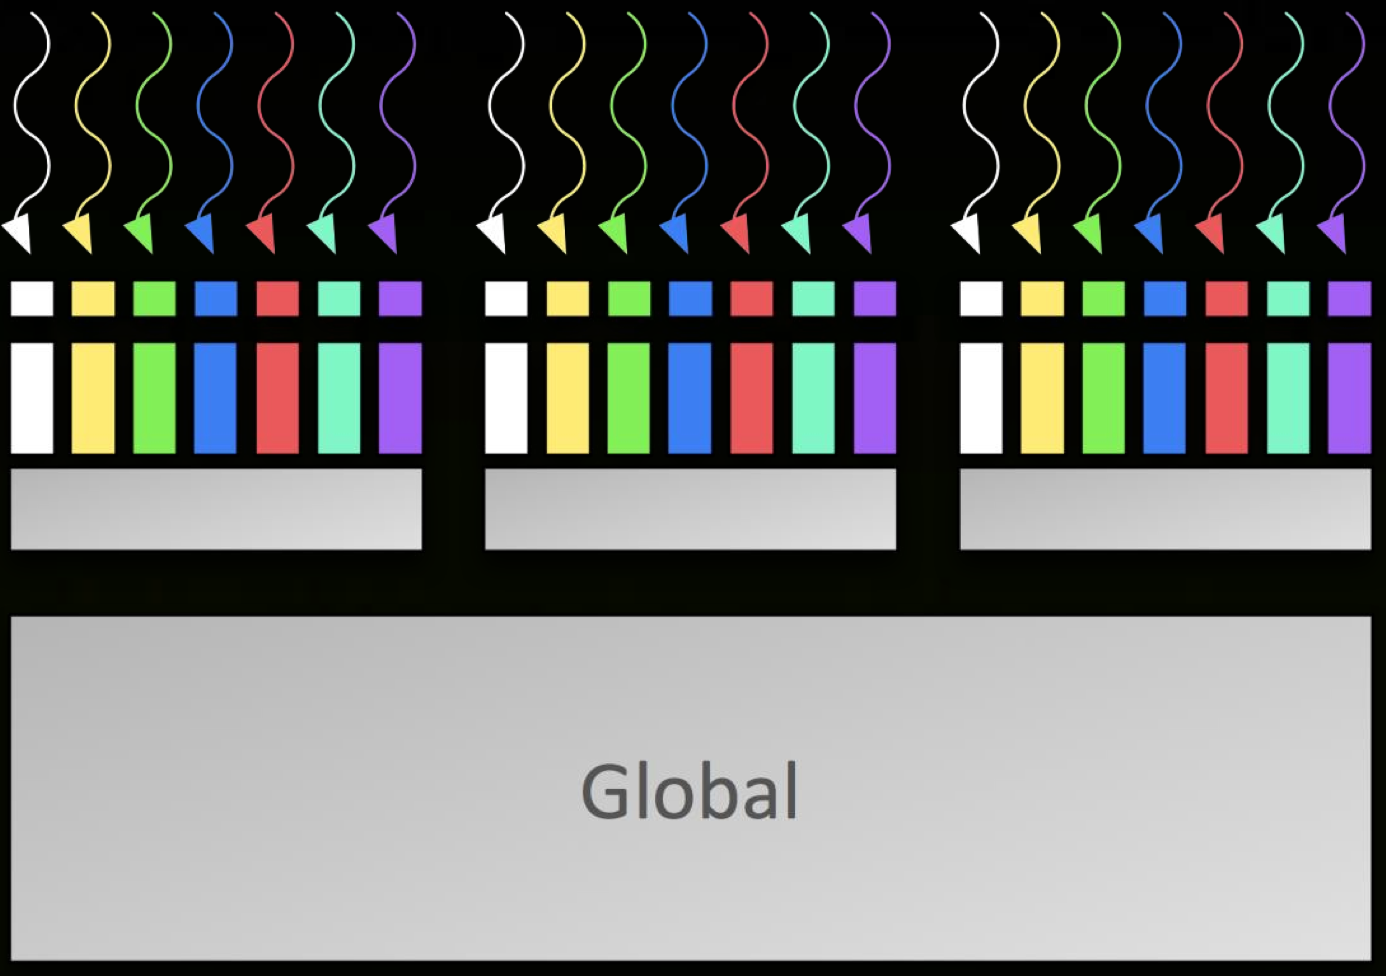
\includegraphics[scale=0.3]{img/cuda-mem}
  \caption{CUDA's memory hierarchy. The small lines represent threads, each of which have their own register (the small
  block) and local memory (the larger block). Each block of threads then have their own shared memory which then feeds
  into the global memory.~\cite{slides:KhronosOpenCLOverview}}
\label{fig:cuda-mem}
\end{figure}

% subsubsection overview_of_cuda (end)

% subsection general_purpose_computing_on_gpus_or_gpgpu (end)

% section differences_in_programming_the_gpu (end)


\section{How the multi-core CPU and GPU can work together} % (fold)
\label{sec:parallelism_in_the_multi_core_cpu_and_gpu}

\subsection{Heterogeneous computing} % (fold)
\label{sub:heterogeneous_computing}
As touched on briefly in~\sectref{sec:differences_in_programming_the_gpu}, heterogeneous computing essentially refers
to systems where there is more than just a single type of processor available~\cite{web:AMDHeteroComp}. This is
arguably most common in consumer desktops and laptops that have both a CPU and GPU component, whether they be on the
same chip or discrete components, so heterogeneous computing as a concept should not be so foreign a concept to most modern
computer users. To make the best use of these different types of processors available in the system, a program can be split
into discrete sections of code, each of which is to be executed by a various processor of which is optimised to run that particular
section of code. Sticking with the GPU and CPU heterogeneous computing example, a program could be split into serial sections
and parallel sections of code, with the serial sections being executed on the CPU and setting up the parallel sections to
run in parallel on the GPU. An example of how CUDA facilitates this can be seen in~\figref{fig:cuda-hetero}. This very much
reflects what was previously stated in~\sectref{sub:why_programs_aren_t_written_just_for_gpus_rather_than_cpus} regarding
how not all tasks can simply be parallelised, and thus depend on certain events happening in sequence first. As this is
very much a reality in modern computer systems, the use of heterogeneous computing systems provides an elegant solution
to the problem, putting differently optimised resources to use.

\begin{figure}[ht]
  \centering
  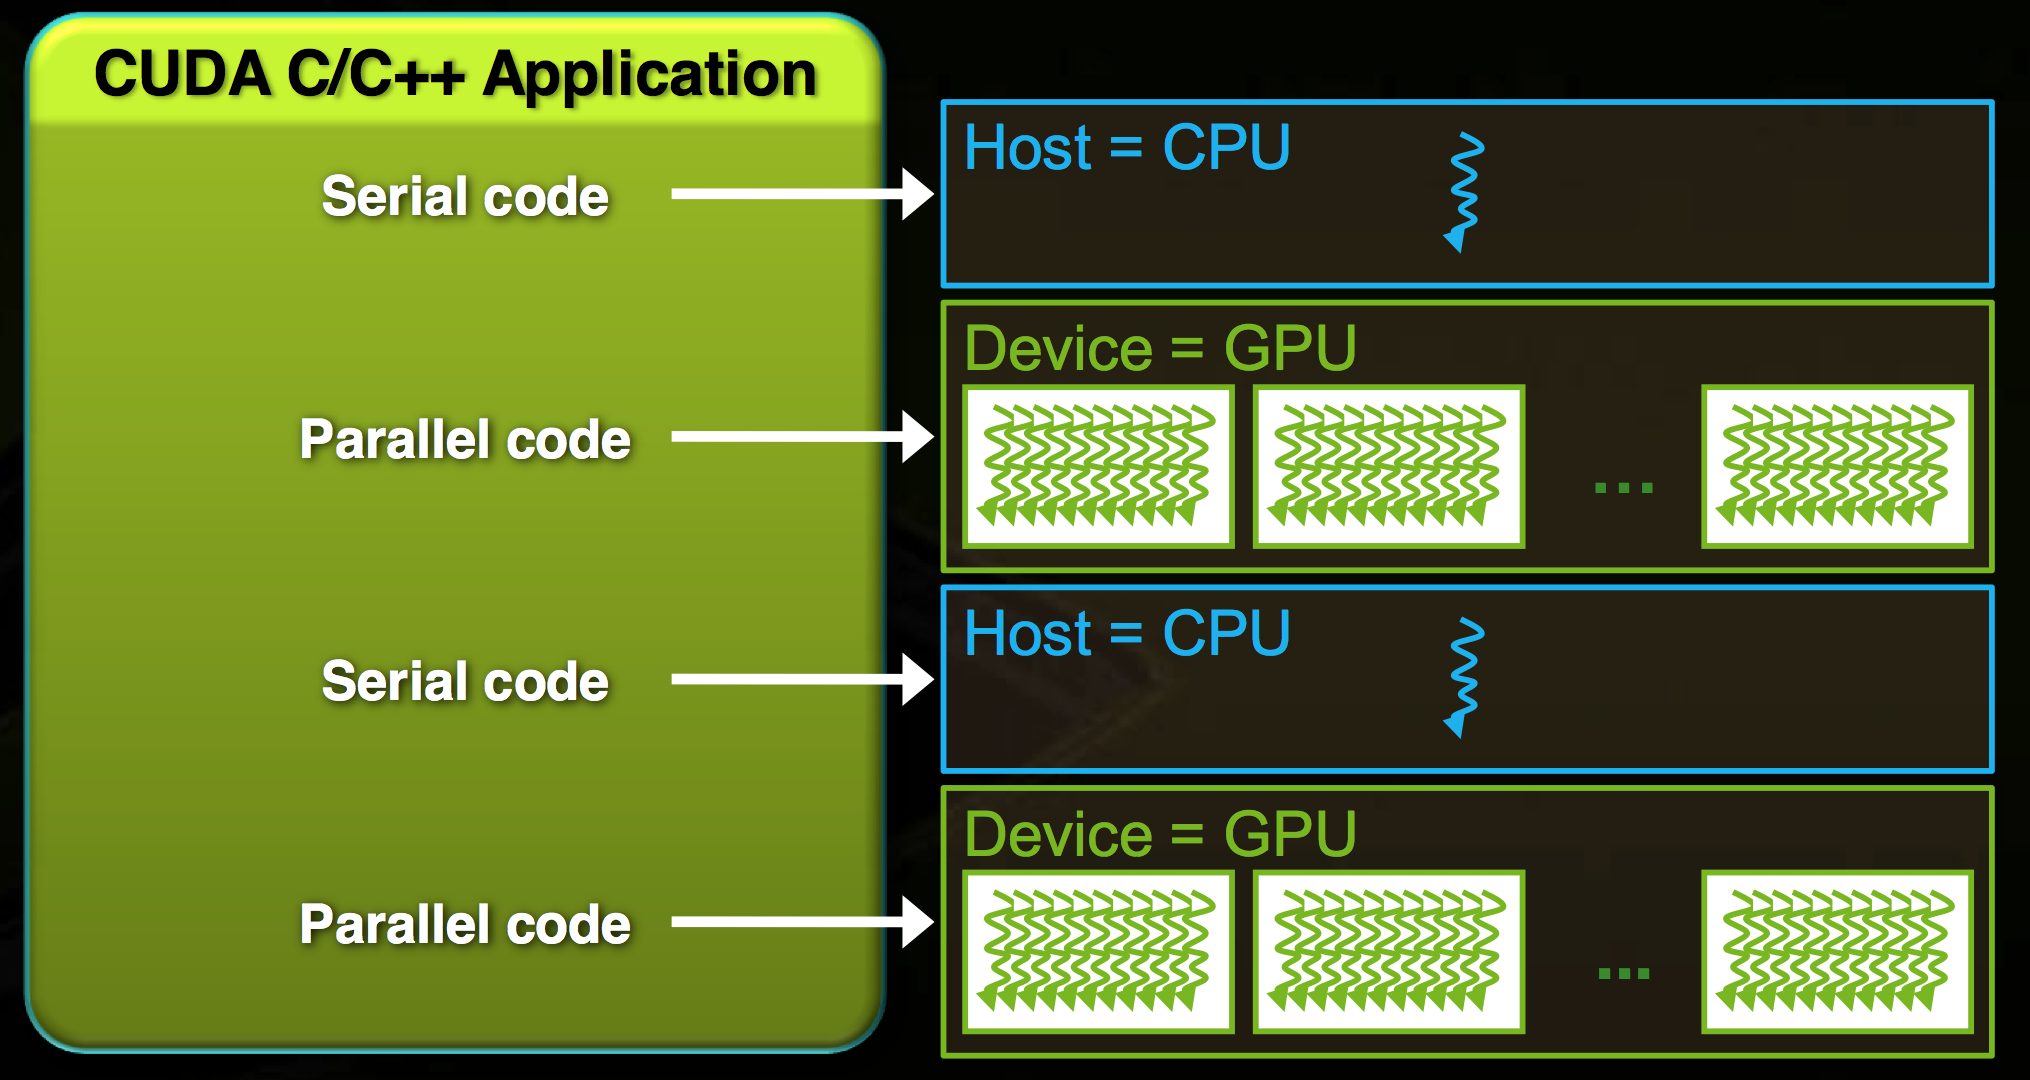
\includegraphics[scale=0.3]{img/cuda-hetero}
  \caption{How CUDA attempts to facilitate heterogeneous computing, splitting the application into serial and parallel
  code sections and executing them on the devices most appropriate for each.~\cite{slides:KhronosOpenCLOverview}}
\label{fig:cuda-hetero}
\end{figure}

% subsection heterogeneous_computing (end)

\subsection{Worked example of heterogeneous computing} % (fold)
\label{sub:worked_example_of_heterogeneous_computing}
To give an example of how a multi-core CPU and GPU can be used together in the one system to optimise performance, we
can look at our earlier shown example of a parallel algorithm for multiplying matrices (shown in~\algoref{algo:matrix_mult_para}
in~\sectref{sub:example_of_a_vs}).

There are many possible ways this algorithm could be split into different parallel and serial parts to be run on the GPU
and CPU, respectively. The most simple way to demonstrate it would be having most of the algorithm run on a specific core
of the CPU, until the ``calculateDotProducts()'' function is treated as a kernel --- to use OpenCL/CUDA terminology ---
and having many $n$ number of executions of this kernel running on the GPU in parallel, where $n$ is the number of dot
products. These dot product calculations, as they are completely independent of other data, would greatly benefit from
being executed on the highly parallel GPU, which the sequential parts of the algorithm, outside of the ``calculateDotProducts()''
kernel, would benefit from being run on the more sequentially optimised CPU. As the number of dot products in matrix
multiplications can get rather large, far larger than say the number of CPU cores present in any consumer CPU, these
dot products could most likely easily be split amongst the hundreds, or even thousands, of GPU cores available. Furthermore,
the simple multiplications and addition operations involved in performing a dot product is by no means a complicated
task for a GPU core to perform.
% subsection worked_example_of_heterogeneous_computing (end)

% section parallelism_in_the_multi_core_cpu_and_gpu (end)


\section{Conclusion} % (fold)
Through looking at graphics processing units (GPUs) and variable-core central processing units (CPUs), we can see how
they both vary considerably in underlying hardware architecture and general use-cases. Through the concept of heterogeneous
computing, it is clear how they
\label{sec:conclusion}

% section conclusion (end)


\bibliographystyle{acm}
\bibliography{report}

\end{document}
